\documentclass[tikz,border=3mm]{standalone}

\usepackage{tikz}
\usetikzlibrary{arrows.meta,positioning,fit,backgrounds,calc,babel}

\begin{document}
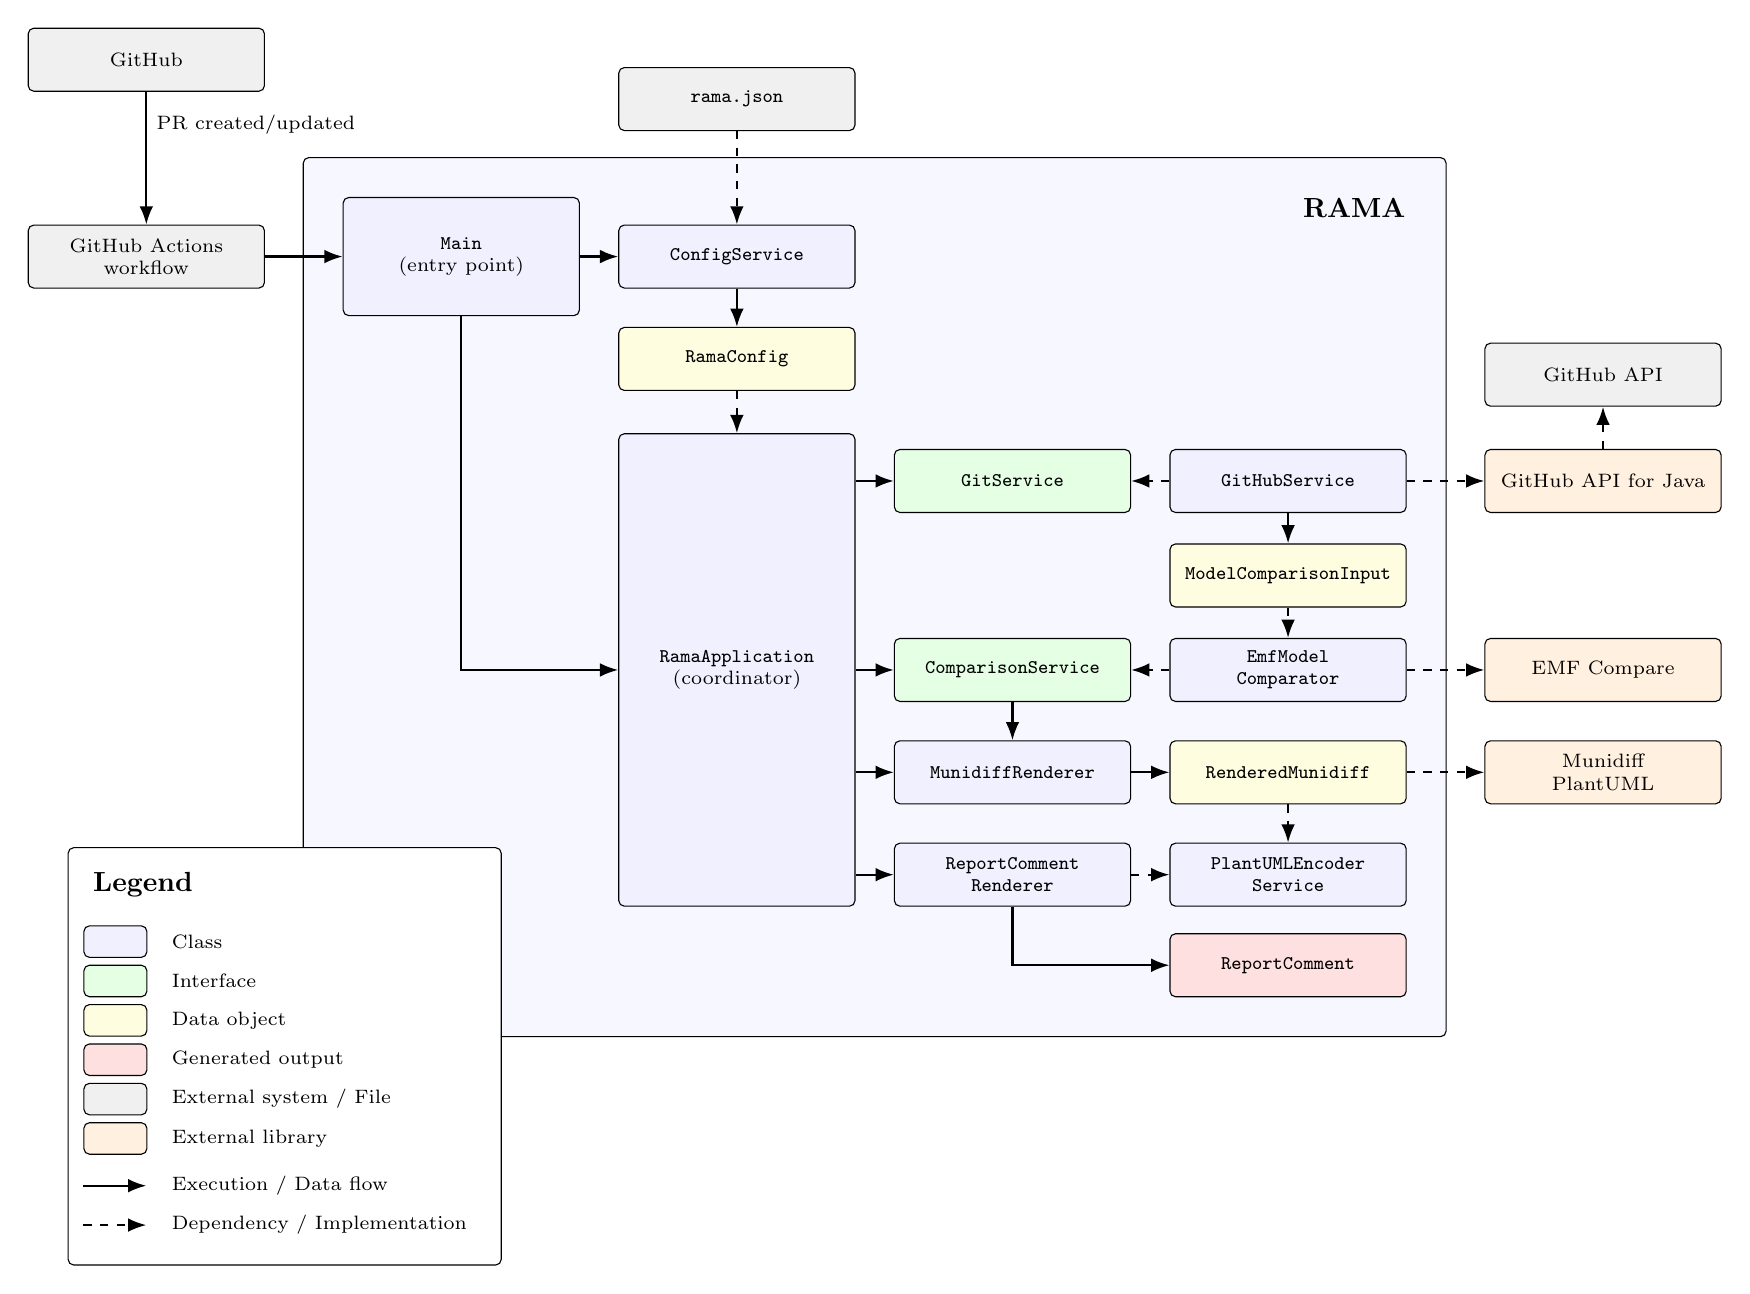
\begin{tikzpicture}[
    font=\scriptsize,
    block/.style={
        draw,
        rounded corners=2pt,
        align=center,
        minimum width=30mm,
        minimum height=8mm,
        inner sep=3pt,
        fill=white
    },
    component/.style={block, fill=blue!6},
    main/.style={component, minimum height=15mm},
    coordinator/.style={component, minimum height=60mm},
    interface/.style={block, fill=green!10},
    data/.style={block, fill=yellow!12},
    output/.style={block, fill=red!12},
    external/.style={block, fill=gray!12},
    library/.style={block, fill=orange!12},
    container/.style={
        draw,
        rounded corners=2pt,
        inner sep=5mm,
        fill=blue!3
    },
    flow/.style={-{Latex}, thick},
    dependency/.style={-{Latex}, thick, dashed}
]

\node[external] (github) at (-4,10.0) {GitHub};
\node[external] (actions) at (-4,7.5) {GitHub Actions\\workflow};
\node[main] (main) at (0.0,7.5) {\texttt{Main}\\(entry point)};
\node[external] (ramaJson) at (3.5,9.5) {\texttt{rama.json}};
\node[component] (configService) at (3.5,7.5) {\texttt{ConfigService}};
\node[data] (ramaConfig) at (3.5,6.2) {\texttt{RamaConfig}};

\node[coordinator] (app) at (3.5,2.25) {\texttt{RamaApplication}\\(coordinator)};

\node[interface] (gitService) at (7.0,4.65) {\texttt{GitService}};
\node[component] (githubService) at (10.5,4.65) {\texttt{GitHubService}};
\node[library] (githubApiForJava) at (14.5,4.65) {GitHub API for Java};
\node[external] (githubApi) at (14.5,6.0) {GitHub API};
\node[data] (input) at (10.5,3.45) {\texttt{ModelComparisonInput}};

\node[interface] (comparisonService) at (7.0,2.25) {\texttt{ComparisonService}};
\node[component] (emfComparator) at (10.5,2.25) {\texttt{EmfModel}\\\texttt{Comparator}};
\node[library] (emf) at (14.5,2.25) {EMF Compare};

\node[component] (munidiffRenderer) at (7.0,0.95) {\texttt{MunidiffRenderer}};
\node[data] (renderedMunidiff) at (10.5,0.95) {\texttt{RenderedMunidiff}};
\node[library] (munidiff) at (14.5,0.95) {Munidiff\\PlantUML};

\node[component] (reportRenderer) at (7.0,-0.35) {\texttt{ReportComment}\\\texttt{Renderer}};
\node[component] (encoder) at (10.5,-0.35) {\texttt{PlantUMLEncoder}\\\texttt{Service}};
\node[output] (reportComment) at (10.5,-1.5) {\texttt{ReportComment}};

\node[
    draw,
    rounded corners=2pt,
    fill=white,
    align=left,
    anchor=north west,
    inner sep=4pt,
    minimum width=55mm,
    minimum height=53mm
] (legendBox) at (-5.0,0.0) {};
\node[font=\bfseries, anchor=north west] at ($(legendBox.north west)+(2mm,-2mm)$) {Legend};

\node[component, minimum width=8mm, minimum height=4mm, anchor=west] at ($(legendBox.north west)+(2mm,-12mm)$) {};
\node[anchor=west] at ($(legendBox.north west)+(12mm,-12mm)$) {Class};

\node[interface, minimum width=8mm, minimum height=4mm, anchor=west] at ($(legendBox.north west)+(2mm,-17mm)$) {};
\node[anchor=west] at ($(legendBox.north west)+(12mm,-17mm)$) {Interface};

\node[data, minimum width=8mm, minimum height=4mm, anchor=west] at ($(legendBox.north west)+(2mm,-22mm)$) {};
\node[anchor=west] at ($(legendBox.north west)+(12mm,-22mm)$) {Data object};

\node[output, minimum width=8mm, minimum height=4mm, anchor=west] at ($(legendBox.north west)+(2mm,-27mm)$) {};
\node[anchor=west] at ($(legendBox.north west)+(12mm,-27mm)$) {Generated output};

\node[external, minimum width=8mm, minimum height=4mm, anchor=west] at ($(legendBox.north west)+(2mm,-32mm)$) {};
\node[anchor=west] at ($(legendBox.north west)+(12mm,-32mm)$) {External system / File};

\node[library, minimum width=8mm, minimum height=4mm, anchor=west] at ($(legendBox.north west)+(2mm,-37mm)$) {};
\node[anchor=west] at ($(legendBox.north west)+(12mm,-37mm)$) {External library};

\draw[flow] ($(legendBox.north west)+(2mm,-43mm)$) -- ($(legendBox.north west)+(10mm,-43mm)$);
\node[anchor=west] at ($(legendBox.north west)+(12mm,-43mm)$) {Execution / Data flow};

\draw[dependency] ($(legendBox.north west)+(2mm,-48mm)$) -- ($(legendBox.north west)+(10mm,-48mm)$);
\node[anchor=west] at ($(legendBox.north west)+(12mm,-48mm)$) {Dependency / Implementation};

\begin{pgfonlayer}{background}
    \node[container, fit=(main)(configService)(ramaConfig)(app)(gitService)(githubService)(input)(comparisonService)(emfComparator)(munidiffRenderer)(renderedMunidiff)(reportRenderer)(encoder)(reportComment)] (ramaBox) {};
\end{pgfonlayer}
\node[font=\bfseries, anchor=north east] at ($(ramaBox.north east)+(-4mm,-4mm)$) {RAMA};

\draw[flow] (github.south) -- node[pos=0.25, right] {PR created/updated} (actions.north);
\draw[flow] (actions.east) -- (main.west);
\draw[flow] (main.south) |- (app.west);
\draw[flow] (main.east) -- (configService.west);

\draw[dependency] (ramaJson.south) -- (configService.north);
\draw[flow] (configService.south) -- (ramaConfig.north);
\draw[dependency] (ramaConfig.south) -- (app.north);

\draw[flow] ($(app.east |- gitService.west)$) -- (gitService.west);
\draw[dependency] (githubService) -- node[above] {} (gitService);
\draw[dependency] (githubService) -- (githubApiForJava);
\draw[dependency] (githubApiForJava) -- (githubApi);
\draw[flow] (githubService.south) -- (input.north);

\draw[flow] ($(app.east |- comparisonService.west)$) -- (comparisonService.west);
\draw[dependency] (input.south) -- (emfComparator.north);
\draw[dependency] (emfComparator) -- node[above] {} (comparisonService);
\draw[dependency] (emfComparator) -- (emf);

\draw[flow] ($(app.east |- munidiffRenderer.west)$) -- (munidiffRenderer.west);
\draw[flow] (comparisonService.south) -- (munidiffRenderer.north);
\draw[flow] (munidiffRenderer) -- (renderedMunidiff);
\draw[dependency] (renderedMunidiff.east) -- (munidiff.west);

\draw[flow] ($(app.east |- reportRenderer.west)$) -- (reportRenderer.west);
\draw[dependency] (renderedMunidiff.south) -- (encoder.north);
\draw[dependency] (reportRenderer) -- (encoder);
\draw[flow] (reportRenderer.south) |- (reportComment.west);

\end{tikzpicture}
\end{document}
